\documentclass[16pt]{beamer}
\usepackage[utf8]{inputenc}
\usepackage{animate}
\usepackage{media9}
\usepackage{amsmath}
\usepackage{amsfonts}
\usepackage{amssymb}
\usepackage{amsthm}
\usepackage{graphicx,epsfig}
\usepackage{float}
 
\usetheme{Madrid}
\usecolortheme{beaver}
\graphicspath{ {images/} }

\newcommand{\calP}{\mathcal{P}}

\usepackage{anyfontsize}
 
%Information to be included in the title page:
\title[Spectral Stability of Multi-Pulses via the Krein Matrix]{Multi-Pulse Stability}
\author[R. Parker]{Ross Parker, Todd Kapitula, Bj{\"o}rn Sandstede}
% \institute{Brown University, Calvin College}
\date{8 November, 2018}

\AtBeginSection[]
{
  \begin{frame}
    \frametitle{Outline}
    \tableofcontents[currentsection]
  \end{frame}
}
 
\begin{document}
 
\frame{\titlepage}
 
\begin{frame}
\frametitle{Outline}
\tableofcontents
\end{frame}

\section{Chen-McKenna Suspension Bridge Equation}

\begin{frame}
	\frametitle{Suspension Bridge Equation}
	\begin{itemize}   
		\item Model for waves on a suspended beam (Chen and McKenna, 1997)

     	\[ u_{tt} + u_{xxxx} + u^+ - 1 = 0 \]

		\item ``I observed that the suspended structure of the bridge was undulating vertically in a wavelike motion of considerable amplitude... The truss would be quiet for a second, and then in the distance one could see a running wave of several nodes approaching.'' \textendash \: R.G.Cone, Chief Engineer (9 February, 1938)
	\end{itemize}
\end{frame}

\begin{frame}
	\frametitle{Suspension Bridge Equation}   
	\begin{itemize}
		\item Model for waves on a suspended beam (Chen and McKenna, 1997)
            \[ u_{tt} + u_{xxxx} + u^+ - 1 = 0 \]
        \item Smooth approximation
            \[ u_{tt} + u_{xxxx} + e^{u} - 1 = 0 \]
        \item In co-moving frame with speed $c$
            \[ u_{tt} - 2 c u_{x t} + u_{xxxx} + c^2 u_{xx} + e^{u} - 1 = 0 \]
	\end{itemize}
\end{frame}

\begin{frame}
	\frametitle{Equilibrium Solutions}   
	\begin{itemize}
		\item Equilibrium solution satisfies ODE
            \[ u_{xxxx} + c^2 u_{xx} + e^{u} - 1 = 0 \]
        \item Linearization about solution $u^*$
            \[ A_0(u^*) = \partial_x^4 + c^2 \partial_x^2 + e^{u^*} \]
        \item Eigenvalues of linearization about 0, for $c \in (0, \sqrt{2})$
            \[ \mu = \pm \sqrt{\frac{-c^2 \pm \sqrt{c^4 - 4}}{2} } = \pm \alpha \pm \beta i \]
	\end{itemize}
\end{frame}

\begin{frame}
	\frametitle{Homoclinic Orbits}   
    \begin{theorem}[van den Berg et. al., 2018] For $c^2 \in [0.5, 1.9]$, a primary pulse solution $q(x)$ exists which is smooth, even, and decays exponentially.
    \end{theorem}
\end{frame}

\begin{frame}
	\frametitle{Homoclinic Orbits}   
    \begin{theorem}[van den Berg et. al., 2018] For $c^2 \in [0.5, 1.9]$, a primary pulse solution $q(x)$ exists which is smooth, even, and decays exponentially.
    \end{theorem}
    Primary pulse solutions $q(x)$ constructed numerically using the string method (Chamard, 2011).

	\begin{figure}
	\begin{center}
	\includegraphics[width=5cm]{images/single1354.eps}
	\includegraphics[width=5cm]{images/single14.eps}
	\caption{Primary pulse solutions, $c = 1.354$ (left) and $c = 1.40$ (right).}
	\label{fig:single1}
	\end{center}
	\end{figure}
\end{frame}

\begin{frame}
\frametitle{Multi-Pulses}   
    \begin{theorem}[Sandstede, 1997]
    \begin{itemize}
	   	\item For $n \geq 2$, an $n-$pulse solution $q_n(x)$ exists which resembles $n$ copies of the primary pulse $q(x)$ separated by distances $X_1, \dots, X_{n-1}$, where 
	    \[ X_j \approx \frac{2 \pi}{\beta} k_j + C \]
	    and $k_j$ is a sufficiently large integer.

    	\item The linearization $A_0(q_n)$ has precisely $n$ real eigenvalues $\nu_1, \dots, \nu_n$ close to 0. 

    	\item $\nu_n = 0$ is a simple eigenvalue, and for $j = 1, \dots, n-1$,
        \begin{align*}
            \nu_j < 0 \text{ if } k_j \text{ is odd} \\
            \nu_j > 0 \text{ if } k_j \text{ is even} 
        \end{align*}
    \end{itemize}
    \end{theorem}
\end{frame}

\begin{frame}
\frametitle{Multi-Pulses} 
    Multi-pulse solutions $q_n(x)$ constructed using Matlab's \texttt{fsolve}.
    \begin{figure}
    \begin{center}
    \includegraphics[width=5cm]{images/double12_12.eps}
    \includegraphics[width=5cm]{images/double12_34.eps}
    \caption{First four 2-pulse solutions, $c = 1.2$.}
    \end{center}
    \end{figure}
\end{frame}

\begin{frame}
\frametitle{PDE eigenvalue problem} 

	\begin{itemize}
	\item Linearization of the suspension bridge PDE about $q_n(x)$ is the quadratic $\star$-even operator polynomial eigenvalue problem

    \[ \calP_2(\lambda; q_n)v = [A_2 \lambda^2 + A_1 \lambda + A_0(q_n)]v = 0 \]

    \begin{align*}
    A_0(q_n) &= \partial_x^4 + c^2 \partial_x^2 + e^{q_n} \\
    A_1 &= -2 c \partial_x \\
    A_2 &= I
    \end{align*}

    \item $A_0$ has $n$ eigenvalues close to 0.
	\end{itemize}
\end{frame}

\section{Krein Matrix Approximation}

\begin{frame}
\frametitle{Krein Matrix}
\begin{definition}[Kapitula et. al., 2019]
    The \emph{Krein matrix} is an $n \times n$ matrix-valued function $K_S(z)$ associated with 
    \begin{itemize}
    	\item A $\star$-even operator polynomial 
    	\[
    	\calP_n(\lambda) = \sum_{j=0}^n \lambda^j A_j
    	\] 
    	with operator coefficients $A_j$ in a Hilbert space $X$
    	\item A finite dimensional subspace $S \subset X$.
    \end{itemize}

    The \emph{Krein eigenvalues} are the eigenvalues $r_1(z), \dots, r_n(z)$ of $K_S(z)$.
    \begin{itemize}
      \item $r_j(z)$ is meromorphic.
      \item If $\lambda = iz$ is a polynomial eigenvalue, then 
      either some $r_j(z) = 0$ or the corresponding eigenfunction is in $S^\perp$.
      \item The Krein signature of $\lambda = i z$ can be determined by the slope of the graph of a Krein eigenvalue $r_j(z)$.
    \end{itemize}
\end{definition}
\end{frame}

\begin{frame}
\frametitle{Krein Matrix Construction}
	To construct the Krein matrix, we need
	\begin{itemize}
		\item A $\star$-even operator polynomial $\calP_n(\lambda)$
		\item A finite dimensional subspace $S$ of $X$ spanned by $s_1, \dots, s_n$
	\end{itemize}

	The Krein matrix is the $n \times n$ matrix $K_S(z)$ with entries

        \begin{align*}
        [K_S&(z)]_{jk} = -z \Big( 
        \langle s_j , \calP_n(iz)s_k\rangle \\
        &- \langle s_j , \calP_n(iz) P_{S^{\perp}} (P_{S^{\perp}} \calP_n(iz)|_{S^{\perp}} )^{-1} P_{S^{\perp}} \calP_n(iz) s_k \rangle \Big)
        \end{align*}

    The choice of an appropriate $S$ is critical.
\end{frame}

\begin{frame}
\frametitle{Krein Matrix Approximation}
	Consider the following scenario. 
	\begin{itemize}	
	\item We have a $\star$-even operator polynomial
	\[ \calP_2(\lambda) = A_2 \lambda^2 + A_1 \lambda + A_0 \]
	\item $A_0$ has $n$ eigenvalues near 0 with corresponding eigenfunctions $\{s_1, \dots, s_n \}$
	\item Let $S$ be the $n-$dimensional space spanned by these
	\end{itemize}
\end{frame}

\begin{frame}
\frametitle{Krein Matrix Approximation}
	The Krein matrix is given by
	\begin{align*}
        [K(z)]_{jk} &= -z \Big( 
        \langle s_j , \calP_2(iz)s_k\rangle \\
        &- \langle s_j , \calP_2(iz) P_{S^{\perp}} (\underbrace{P_{S^{\perp}} \calP_2(iz)|_{S^{\perp}} }_{\text{This depends on }z})^{-1} P_{S^{\perp}} \calP_2(iz) s_k \rangle \Big) \\
        p_2(iz) &= -A_2 z^2 + i A_1 z + A_0
    \end{align*}

    \begin{itemize}
    \item<1-> Idea: For small $z$, approximate $\calP_2(iz)$ by $A_0$ in the term $(P_{S^{\perp}} \calP_2(iz)|_{S^{\perp}})^{-1}$
    \item<2-> $A_0$ is invertible on $S^\perp$ by our choice of $S$.
    \item<2-> We have a nice bound on $(P_{S^{\perp}} A_0|_{S^{\perp}})^{-1}$
	\end{itemize}
\end{frame}

\begin{frame}
\frametitle{Krein Matrix Approximation}
	\begin{lemma}[Kapitula et. al., 2019]
	\begin{itemize}
	\item Consider the quadratic $\star$-even operator polynomial
	\[ \calP_2(\lambda) = A_2 \lambda^2 + A_1 \lambda + A_0 \]
	\item Suppose $A_0$ has $n$ eigenvalues near 0 with corresponding eigenfunctions $\{s_1, \dots, s_n \}$, and let $S$ be the $n-$dimensional space spanned by these
	\item Then there exists a constant $C_0$ such that for $|\lambda| < C_0$, the Krein matrix is analytic and takes the form
	\begin{align*}
	K_S(z) &= -z\left[ \text{diag}(\mu_1, \dots, \mu_n) - K_1 i \overline{z} - K_2 \overline{z}^2 + \mathcal{O}(|z|^3)\right] \\
	K_1(z)_{jk} &= \langle s_j, A_1 s_k\rangle \\
	K_2(z)_{jk} &= \langle s_j, A_2 s_k\rangle -
	\langle s_j, A_1 P_{S^{\perp}} (P_{S^{\perp}} A_0)|_{S^{\perp}} )^{-1} P_{S^{\perp}} A_1 s_k \rangle \Big)
	\end{align*}
    \end{itemize}

	\end{lemma}
\end{frame}

\section{Spectral Stability of Multi-Pulse Solutions to Suspension Bridge Equation}

\begin{frame}
\frametitle{Polynomial Eigenvalue Problem}
	\begin{itemize}
	\item Linearization of the suspension bridge equation about an $n-$pulse solution $q_n$ is the quadratic $\star$-even operator polynomial

    \begin{align*}
    P_2(\lambda; q_n)v &= [A_2 \lambda^2 + A_1 \lambda + A_0(q_n)]v = 0 \\
    A_0(q_n) &= \partial_x^4 + c^2 \partial_x^2 + e^{q_n} \\
    A_1 &= -2 c \partial_x \\
    A_2 &= I
    \end{align*}

    \item $A_0(q_n)$ has $n$ eigenvalues $\nu_1, \dots, \nu_n$ near 0

    \item Choose $S$ to be the span of the corresponding eigenfunctions $s_1, \dots, s_n$
	\end{itemize}
\end{frame}

\begin{frame}
\frametitle{Essential Spectrum}
	Essential spectrum is purely imaginary and bounded away from the origin, and does not depend on the solution we are linearizing about.
	\[ \sigma_{ess} = [ (-\infty, r] \cup [r, \infty) ]i \]
	where $r$ depends on the speed $c$.
	\begin{figure}
	\begin{center}
	\includegraphics[width=6cm]{images/essspecboundary.eps}
	\caption{Essential spectrum boundary $r$ as a function of traveling wave speed $c$.}
	\end{center}
	\end{figure}
\end{frame}

\begin{frame}
\frametitle{Krein Matrix}
	\begin{theorem}[Kapitula et. al., 2019]
	Let $q_n(x)$ be an $n-$pulse equilibrium solution to the suspension bridge equation with associated lengths $X_1, \dots, X_{n-1}$. Let $\nu_1, \dots, \nu_n$ be the small eigenvalues of $A_0(q_n)$. Then, under some mild hypotheses, the Krein matrix is diagonally dominant and is given by

    \begin{align*}\label{Kreinapprox}
    K_S(z) = ||&q_x||^2 \text{diag} (\nu_1, \dots, \nu_n) \\
     &+ d''(c) I \overline{z}^2 + \mathcal{O}(e^{-(3 \alpha/2) X_m}|z| + |z|^3)
    \end{align*}

    where

    \begin{align*}
    d''(c) &= -\frac{\partial}{\partial c} \left( c ||q_x||^2 \right) \\
    X_m &= \min\{ X_1, \dots, X_{n-1} \} 
    \end{align*}
	\end{theorem}
\end{frame}

\begin{frame}
\frametitle{Location of Eigenvalues}
	\begin{itemize}
		\item The signs of the small, nonzero eigenvalues $\nu_j$ of $A_0(q_n)$ are determined by the geometry of the $n-$pulse $q_n$.

		\item The lengths $X_1, \dots, X_{n-1}$ for $q_n$ are given by
		\begin{align*}
		X_j &\approx \frac{2\pi}{\beta} k_j + C && k_j \text{ integer}
	    \end{align*}

    	\item The signs of the $\nu_j$ is determined by the parity of the integers $k_j$. 
        \begin{align*}
            \nu_j < 0 \text{ if } k_j \text{ is odd} \\
            \nu_j > 0 \text{ if } k_j \text{ is even} 
        \end{align*}
	\end{itemize}
\end{frame}

\begin{frame}
\frametitle{Location of Eigenvalues}
	\begin{itemize}
		\item The nonzero polynomial eigenvalues are given by

		\begin{equation*}
      		\lambda_j^\pm = \pm ||q_x|| \sqrt{ \frac{\nu_j}{d''(c)} } + \mathcal{O}(e^{-(3 \alpha/2) X_m})
      	\end{equation*}

      	We assume $d''(c) > 0$.

        \item For each $\nu_j < 0$ ($k_j$ odd), there is a pair of purely imaginary polynomial eigenvalues $\lambda = \pm i \beta_j$.

        \item For each $\nu_j > 0$ ($k_j$ even), there is a pair of real polynomial eigenvalues $\lambda = \pm \beta_j$.
	\end{itemize}
\end{frame}

\begin{frame}
\frametitle{Stability Criterion}
\begin{corollary}[Kapitula et. al., 2019]If $\nu_1, \dots, \nu_{n-1} < 0$ (equivalently, all $k_j$ are odd), there are $n - 1$ pairs of purely imaginary polynomial eigenvalues near 0, thus $q_n$ is linearly neutrally stable.
\end{corollary}
\end{frame}

\begin{frame}
\frametitle{Stability Criterion: Stable 2-pulse}
\begin{figure}
\begin{center}
\includegraphics[width=4.5cm]{images/stable1.eps}
\includegraphics[width=4.5cm]{images/stable1A0.eps}
\includegraphics[width=4.5cm]{images/stable1spec.eps}
\caption{Spectra of $A_0$ and $P_2(\lambda)$ for stable 2-pulse}
\end{center}
\end{figure}
\end{frame}

\begin{frame}
\frametitle{Stability Criterion: Stable 3-pulse}
\begin{figure}
\begin{center}
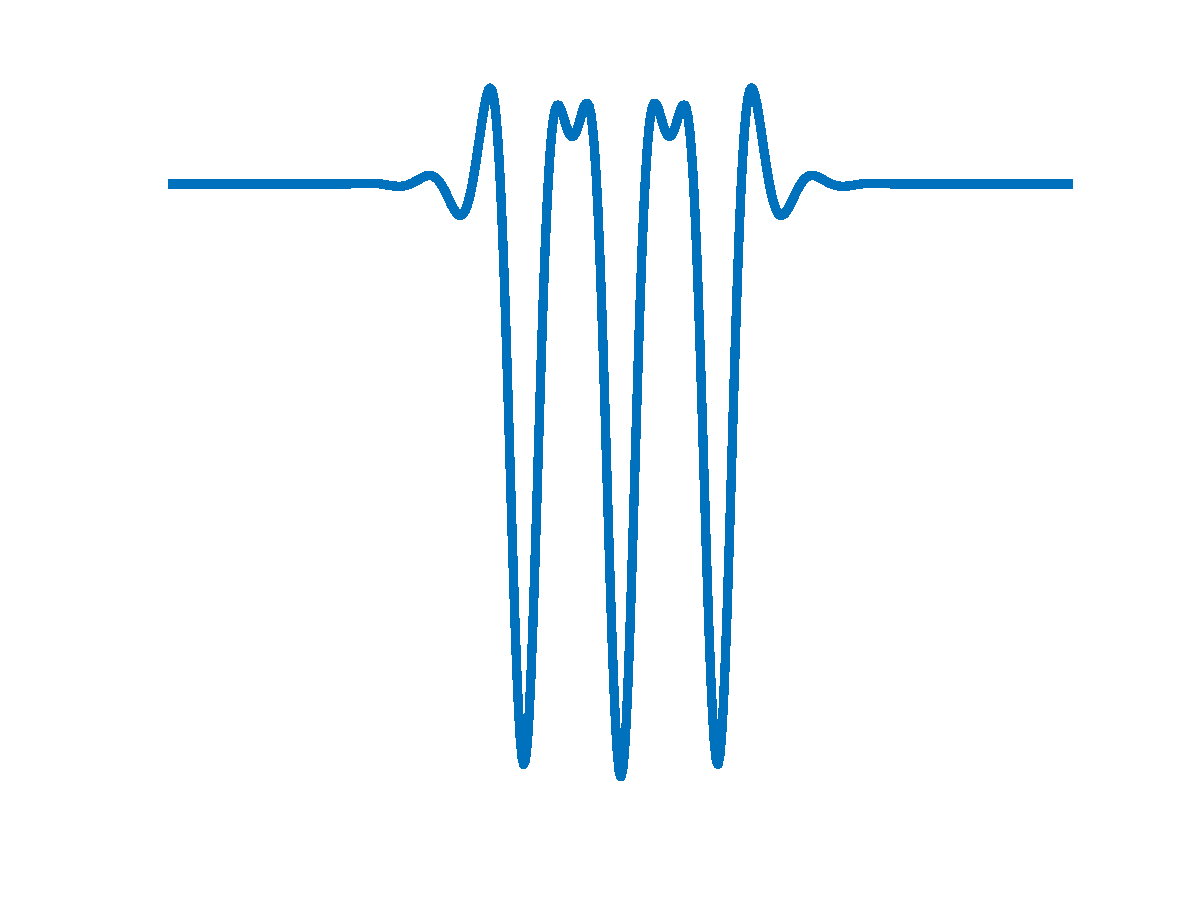
\includegraphics[width=4.5cm]{images/stable2.eps}
\includegraphics[width=4.5cm]{images/stable2A0.eps}
\includegraphics[width=4.5cm]{images/stable2spec.eps}
\caption{Spectra of $A_0$ and $P_2(\lambda)$ for stable 3-pulse}
\end{center}
\end{figure}
\end{frame}

\begin{frame}
\frametitle{Instability Criterion}
\begin{corollary}[Kapitula et. al., 2019]If $\nu_j > 0$ for some $j = 1, \dots, n-1$ (equivalently, at least one $k_j$ is even), then there is at least one polynomial eigenvalue with positive real part, thus $q_n$ is linearly unstable.
\end{corollary}
\end{frame}

\begin{frame}
\frametitle{Instability Criterion: Unstable 2-pulse}
\begin{figure}
\begin{center}
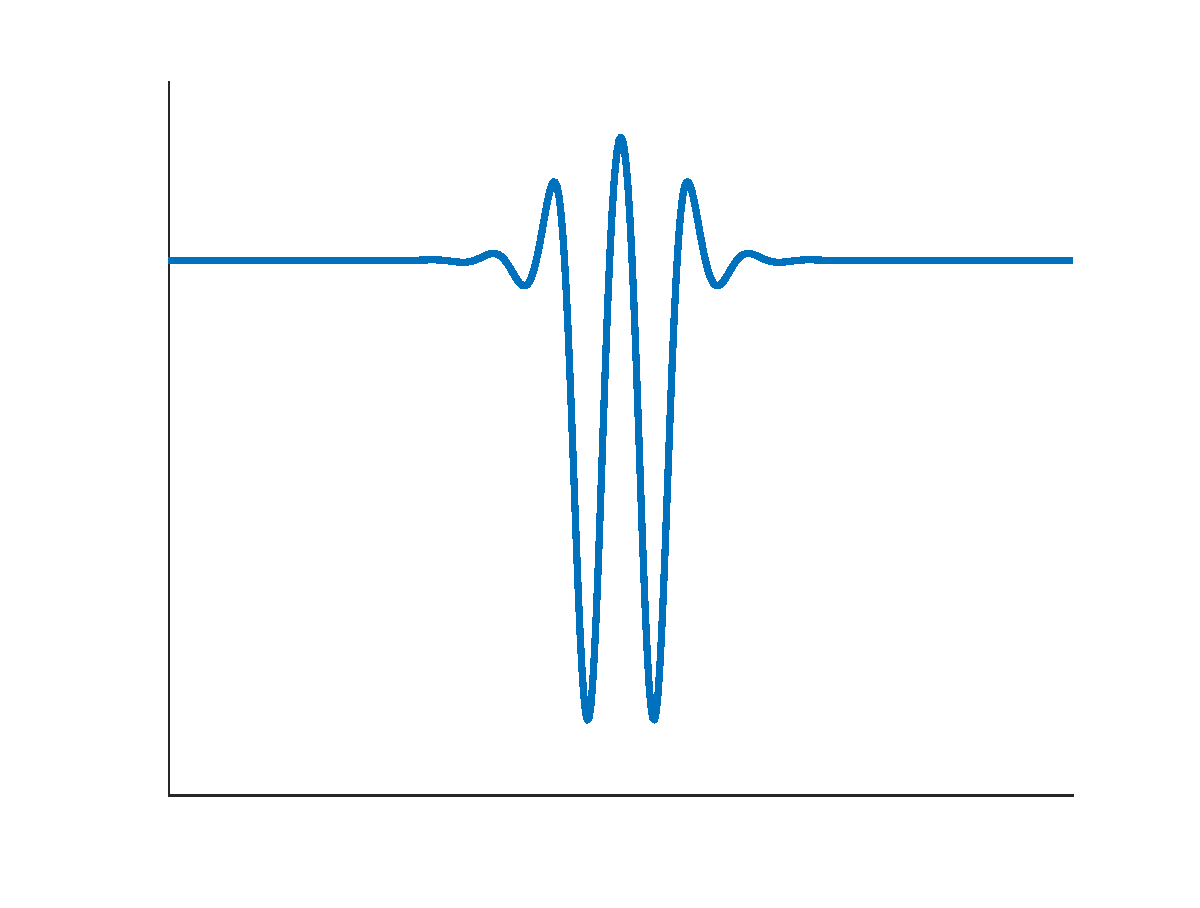
\includegraphics[width=4.5cm]{images/unstable1.eps}
\includegraphics[width=4.5cm]{images/unstable1A0.eps}
\includegraphics[width=4.5cm]{images/unstable1spec.eps}
\caption{Spectra of $A_0$ and $P_2(\lambda)$ for unstable 2-pulse}
\end{center}
\end{figure}
\end{frame}

\begin{frame}
\frametitle{Instability Criterion: Unstable mixed 3-pulse}
\begin{figure}
\begin{center}
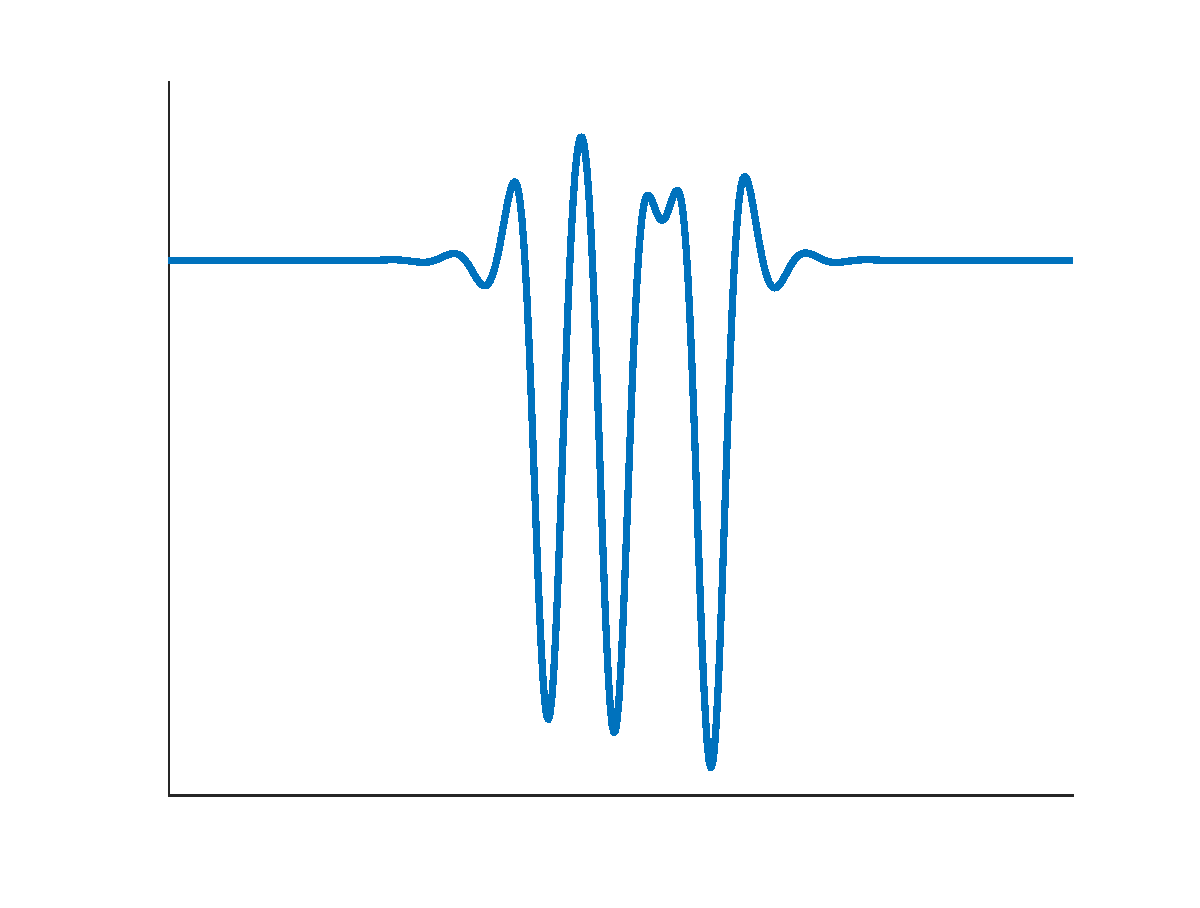
\includegraphics[width=4.5cm]{images/unstable2.eps}
\includegraphics[width=4.5cm]{images/unstable2A0.eps}
\includegraphics[width=4.5cm]{images/unstable2spec.eps}
\caption{Spectra of $A_0$ and $P_2(\lambda)$ for unstable mixed 3-pulse}
\end{center}
\end{figure}
\end{frame}

\begin{frame}
\frametitle{Future Work}
    \begin{itemize}
      \item Explore other applications of the Krein Matrix.
      \item Use Lin's method for stability analysis of multi-pulse solutions to the suspension bridge equation.
    \end{itemize} 
\end{frame}

\begin{frame}
\frametitle{References}
      \fontsize{12}{7.2}\selectfont
      \begin{thebibliography}{9}
      \setbeamertemplate{bibliography item}[text]
      \bibitem{Chamard11} Chamard J. et al. \emph{Computation of minimum energy paths for quasi-linear problems}. J. Sci. Comp., 49 (2011), 180-194.
      \bibitem{Chen97} Chen Y. and McKenna P.J. \emph{Traveling waves in a nonlinearly suspended beam: theoretical results and numerical observations}. J. Diff. Eq., 136 (1997), 325-355.\bibitem{Kap19} Kapitula T. et at. \emph{Another reformulated Krein matrix for star-even polynomial operators with applications}. Submitted for publication, 2019.
      \bibitem{San97} Sandstede B. \emph{Instability of localized buckling modes in a one-dimensional strut model}. Phil. Trans. Roy. Soc. A, 355 (1997), 2083-2097.
      \bibitem{Berg18} van den Berg J.B. et al. \emph{Continuation of homoclinic orbits in the suspension bridge equation: A computer-assisted proof}. J. Diff. Eq., 264 (2018), 3086-3120.
      \end{thebibliography}
\end{frame}



\end{document}